\chapter{Bahnoptimierung}
\label{cha:Bahnoptimierung}
%\cite{Eggers.2019}
%\cite{Engelke.2008}
%\cite{Ziaukas.2017}
%\cite{Hansen.2012}
%\cite{Spong.2020}
Im Folgenden wird die zuvor im Kapitel \ref{sec:trajektorie} eingeführte Bewegungsbahn des Programms $Kleben-Seitenwand$ unter Berücksichtigung der vom Roboter aufgenommenen Energie optimiert. Dazu wird das Optimierungsproblem zunächst definiert, eine passende Zielfunktion aufgestellt und geeignete Nebenbedingungen festgelegt. Anschließend werden der numerische Solver sowie der verwendete Algorithmus beschrieben. Zum Abschluss werden die Ergebnisse der  Optimierung analysiert. 
%
\section{Definition des Optimierungsproblems}
Gegenstand der Optimierung ist die Minimierung des Energieverbrauchs eines KR210 R2700-2 Industrieroboters entlang einer Bewegungsbahn. Im Ziel der Arbeit ist festgelegt, den Ansatz möglichst praktikabel für die Automobilproduktion zu gestalten. Dazu wird der Begriff der Bewegungsbahn weiter eingegrenzt. Es wird unterschieden zwischen prozessbezogenen Bewegungen, z.B. entlang einer Schweißnaht oder Klebebahn, und nicht-prozessbezogenen Bewegungen, z.B. das Anfahren einer Vorposition oder der Home-Position in der Bewegungsart PTP. Im Folgenden werden explizit nicht prozessrelevante Trajektorien betrachtet. Der Ansatz basiert auf der geometrischen Anpassung  der Bewegungsbahn durch einen zu optimierenden Parametervektor $\bm{q}_{v}$. Dieser umfasst die Gelenkwinkel des, nach der Hälfte der Bewegungsdauer definierten Via-Punkts \cite[S~532~ f.]{Ziaukas.2017}.
%
\begin{equation}
	\label{eqn:parametervektor}
	\bm{q}_{v} = [q_{v,1},...,q_{v,6}]^T 
\end{equation}
%
Der Startwert jedes Via-Punkts wird auf der Hälfte der Winkelposition zwischen dem Start- und Zielpunkt definiert.
\begin{equation}
	\label{eqn:parametervektor-startkonfiguration}
	q_{v,i,Start} = \dfrac{q_{s,i}+q_{e,i}}{2} ~\forall~ i \in \{1,...,6\}
\end{equation}
Die Minimierung der Leistungsaufnahme basiert auf der konfigurationsabhängigen Reduktion der Massenträgheitsmomente in $\bm{M}(\bm{q})$, so dass bei gleichbleibender Winkelbeschleunigung die Drehmomente in den Gelenken reduziert werden \cite[S.~531]{Ziaukas.2017}. Das Optimierungsproblem besteht darin, den Parametervektor zu identifizieren, für den die minimale Zielfunktion erreicht wird.
%\begin{equation}
%	\bm{q}_{v,opt} = \argminA_{\bm{q}_{v}} J_{P_{zu}}(\bm{q}_{v}).
%\end{equation}
%
\begin{equation}
	\argminA_{\bm{q}_{v}} J(\bm{q}_{v}) = \{\bm{q}_{v} \mid J(\bm{q}_{v}) = \min_{\bm{q}_{v,opt}} J(\bm{q}_{v,opt})\}.
\end{equation}
%
\section{Zielfunktion}
Für die Definition der Zielfunktion wird angenommen, dass die generatorisch erzeugte Leistung während des Abbremsvorgangs über Bremswiderstände dissipiert \cite[S.~1327]{Pellicciari.2015}. Zur Identifizierung des Optimums werden die Zielfunktionen \ref{eqn:torque}, \ref{eqn:emechges} \cite[S.~1216]{Saravanan.2008} und \ref{eqn:emech} \cite[S.~57]{Eggers.2019} aufgestellt. Die Integrationsgrenzen $t_s$ und $t_e$ entsprechen dem Start- bzw. Zielzeitpunkt. Der Ausdruck \ref{eqn:torque} wird in abgewandelter Form in \cite[S-~1]{Hansen.2012} beschrieben und erzielt durch Quadrieren den Vorteil, dass hohe Drehmomente stärker gewichtet werden. Dabei wird jedoch nicht ersichtlich, ob Leistung aufgenommen oder abgegeben wird.
%
\begin{equation}
	\label{eqn:torque}
	J_{\tau}(\bm{q}_{v}) = \int_{ts}^{te}\sum_{i=1}^{n}\tau_i(t)^2~dt
\end{equation}
%
Von einem Vorschlag der Zielfunktion \ref{eqn:emechges} wird ebenso Abstand genommen, da hierbei die generatorisch umgewandelte Leistung während des Abbremsvorgangs als aufgenommene Leistung der Verbraucher bewertet wird. 
%
\begin{equation}
	\label{eqn:emechges}
	J_{P_{mech_{ges}}}(\bm{q}_{v}) = \int_{ts}^{te}\sum_{i=1}^{n}\left|\tau_i(t)\dot{q_i}\right|^2~dt
\end{equation}
%
Die Zielfunktion \ref{eqn:emech} entspricht dem physikalischen Ausdruck der verrichteten mechanischen Arbeit über die zugeführte Leistung. Es wird ausschließlich die motorisch aufgenommene, mechanische Leistung $P_{mech}>0$ berücksichtigt. 
%
\begin{equation}
	\label{eqn:emech}
	J_{P_{mech_{zu}}}
	(\bm{q}_{v}) 
	= E_{mech}(\bm{q}_{v}) 
	=\int_{ts}^{te}P_{mech_{zu}}(\bm{q}_{v},t)~dt
\end{equation}
%
Die numerische Implementierung der Zielfunktion in  MATLAB\textsuperscript{\textregistered} entspricht der Gleichung  \ref{eqn:numerischezielfunktion}. Die Schrittweite ist in Anlehnung an die Abtastung der Messeinrichtung  mit $\Delta t = 0.004 \text{s}$ festgelegt. Die Anzahl der Schritte $m$  wird gemäß $(t_s-t_e)/\Delta t$ berechnet.
%
\begin{equation}
	\label{eqn:numerischezielfunktion}
	J_{P_{mech_{zu}}}
	(\bm{q}_{v}) 
	= E_{mech}(\bm{q}_{v}) 
	= \sum_{k=1}^{m} P_{mech_{zu}}(\bm{q}_{v},t)~\Delta t
\end{equation}
%
\section{Nebenbedingungen}
\label{sec:Nebenbedingungen}
Die Verfahrzeit bleibt gegenüber der Initialbahn konstant und wird durch den Zielzeitpunkt $t_e$ vorgegeben. 
%Eine Anpassung der Variablen für die maximale relative Geschwindigkeit $vel axis[i]$ und Maximalbeschleunigung $acc axis[i]$ im KRL Programm siehe \cite[S.~532]{Ziaukas.2017} erfolgt nicht.
In \cite[S.~40]{Eggers.2019} bzw. \cite[S.~5]{Hansen.2012} werden die Gelenkwinkel der energieoptimierten Bewegungsbahn in der Robotersteuerung über einen Software-in-the-Loop (SiL) Ansatz berechnet. Dadurch ist die Einhaltung von Drehmoment-, Gelenkwinkel-, Geschwindigkeit- und Beschleunigungsgrenzen entsprechend der Gleichungen \ref{eqn:conpos},\ref{eqn:convel}, \ref{eqn:conacc} und \ref{eqn:contau} gewährleistet. 
%
\begin{equation}
	\label{eqn:conpos}
	q_{i,min} \leq q_{i}(t) \leq q_{i,max}  ~\forall~ i \in \{1,...,6\},~ t \in [t_s;t_e]
\end{equation}
%
\begin{equation}
	\label{eqn:convel}
	\dot{q}_{i,min} \leq \dot{q}_{i}(t) \leq \dot{q}_{i,max}  ~\forall~ i \in \{1,...,6\},~ t \in [t_s;t_e]
\end{equation}
%
\begin{equation}
	\label{eqn:conacc}
	\ddot{q}_{i,min} \leq \ddot{q}_{i}(t) \leq \ddot{q}_{i,max}  ~\forall~ i \in \{1,...,6\}, ~t \in [t_s;t_e]
\end{equation}
%
\begin{equation}
	\label{eqn:contau}
	\tau_{i,min} \leq \tau_{i}(t) \leq \tau_{i,max}  ~\forall~ i \in \{1,...,6\},~ t \in [t_s;t_e]
\end{equation}
%
In der vorliegenden Arbeit sind ausschließlich die Schranken der Gelenkwinkel $q_{v,i}$ im Via-Punkt definiert. Die Formulierung zielt darauf ab, dass die optimierte Bewegungsbahn nicht signifikant von der Initialbahn abweicht \cite[S.~5]{Hansen.2012}.
\begin{equation}
	\label{eqn:Schranken}
	q_{v,i} \in [q_{i,min};q_{i,max}] ~\forall~ i \in \{1,...,6\}
\end{equation}
Grenzwerte für die Drehmomente, Winkelgeschwindigkeiten und Winkelbeschleunigungen werden nicht explizit formuliert.  Im Anschluss an die Optimierung erfolgt eine manuelle Überprüfung der Verläufe.
%
\section{Solver- und Optimierungsalgorithmus}
Die numerische Umsetzung der Optimierung erfolgt unter Verwendung der MATLAB\textsuperscript{\textregistered} Optimization Toolbox\texttrademark. Für das nichtlineare Optimierungsproblem wird anhand einer Entscheidungstabelle in \cite[S.~80]{OptimizationToolbox.2023} der Solver fmincon ausgewählt.  Im Anhang \ref{add:optimierer} ist der implementierte Code aufgeführt. Die Zielfunktion wird mithilfe des inversen Dynamik-Modells in der separaten MATLAB\textsuperscript{\textregistered}-Funktion $calc\_objective(qs,qe,qv,te)$ berechnet, siehe Anhang \ref{add:zielfunktion}. Es sind keine Gleichungs- bzw. Ungleichungssnebenbedingungen definiert. Es ist jedoch möglich, die im letzten Abschnitt beschriebenen Nebenbedingungen zu einem späteren Zeitpunkt hinzuzufügen. Für die einzelnen Via-Punkte des Parametervektors $\bm{q}_{v}$ sind jeweils die obere und untere Schranke entsprechend der Gleichung \ref{eqn:Schranken} festgelegt. Für den Algorithmus wird das Verfahren der sequentiellen quadratischen Programmierung (sequential quadratic programming (SQP)) gewählt.  SQP ist eine Verallgemeinerung des Newton-Verfahren\footnote{Das Newton-Verfahren ist ein numerischer Ansatz zur Lösung nichtlinearer Gleichungssysteme, bei dem eine iterative Approximation mithilfe der nach ersten Glied abgebrochenen Taylorreihe erfolgt \cite[S.~46]{Papageorgiou.2015}.} für beschränkte Problemstellungen \cite[S.~113]{Papageorgiou.2015}. In \cite[S.~253]{OptimizationToolbox.2023} wird beschrieben, dass für jeden Iterationsschritt die Einhaltung der Schranken gewährleistet ist. Diese wird als Vorteil aufgrund der Komplexität  der Inversen-Dynamik zur Berechnung der Zielfunktion  bewertet. Notwendige Bedingungen zur Identifikation eines lokalen Minimums sind die  Karush-Kuhn-Tucker (KKT) Konvergenzkriterien  \cite[S.~321]{Nocedal.2006}.  In jeder Iteration des SQP-Verfahrens wird versucht, die KKT-Bedingungen für das ursprüngliche Problem durch eine quadratische Approximation der Zielfunktion zu erfüllen \cite[S.~337~ff.]{Reinhardt.2013}. Zusätzlich bietet MATLAB\textsuperscript{\textregistered} für fmincon die Option, Konvergenzkriterien zu definieren. Im Rahmen der ersten KKT Bedingung wird der Gradient der Zielfunktion überprüft. Falls dieser Wert nur annähernd Null erreicht, kann ein Schwellenwert festgelegt werden, bei dessen Unterschreitung die erste KKT-Bedingung erfüllt ist. Es ist außerdem möglich, eine maximale Anzahl von Iterationen festzulegen, bei deren Erreichen der Algorithmus beendet wird. Die Variable \lstinline[language=Matlab]|'MaxIterations'| wird mit 25 frei gewählt.  Für eine ausführliche Herleitung von SQP-Algorithmen auf der Basis des Newton-Lagrange-Verfahren wird auf \cite[S.~529~ff.]{Nocedal.2006} verwiesen.
%
\section{Durchführung der Optimierung}
Die Arbeit verfolgt den Anspruch, dass die identifizierten Einsparungen über das Laborumfeld hinaus in der industriellen Praxis realisiert werden können. Dazu wird eine Bewegung der Bewegungsart PTP betrachtet, die in nahezu jedem Programm den Verfahrweg nach Programmende in die Grundstellung abbildet. Exemplarisch wird die Bewegung vom letzten Prozesspunkt zurück in die Grundstellung im Fertigungsprogramm  $Kleben-Seitenwand$  optimiert. Diese wurde bereits im Kapitel Trajektorie-Planung \ref{sec:trajektorie} eingeführt. Die Start- und Zielkonfiguration ist in der Tabelle \ref{tab:simu} aufgeführt.  Im ersten Schritt wird die Initial-Trajektorie abgefahren. Dabei werden die Bewegungsdaten über die RSI-Signalaufzeichnung erfasst. Anhand der Genlenkwinkelgeschwindigkeitsverläufe, siehe Abbildung \ref{fig:winkelgeschwindigkeit_py1} wird die Gesamtbewegungsdauer mit 1,2 s geschätzt. Für die Startwerte \ref{eqn:parametervektor-startkonfiguration} des Parametervektors \ref{eqn:parametervektor} wird die Optimierung in MATLAB\textsuperscript{\textregistered}, siehe Anhang \ref{add:optimierer} ausgeführt. Die Anzahl der Iterationen ist auf 25 beschränkt. In der Abbildung \ref{fig:funktionswerte-iteration} wird deutlich, dass die energieoptimierten Gelenkwinkel bereits nach acht Iterationsschritten näherungsweise erreicht sind.
%
\begin{figure}[tbph]
	\centering
	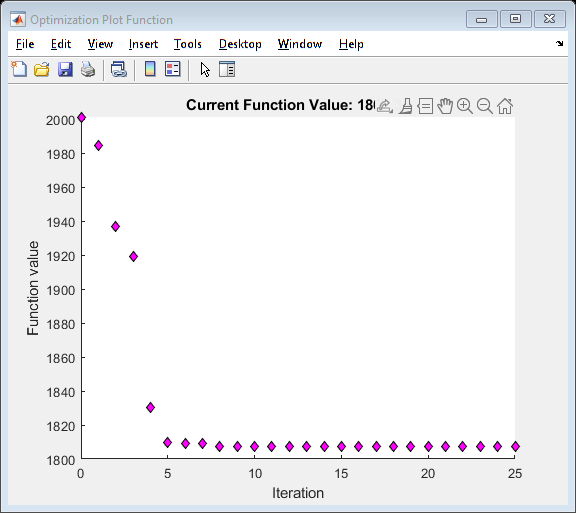
\includegraphics [width=4in]{images/optimization_01}
	\caption{Zielfunktionswerte einzelner Optimierungsiterationen}
	\label{fig:funktionswerte-iteration}
\end{figure}
%
\section{Auswertung der Optimierungsergebnisse}
Die identifizierten, energieoptimierten Via-Punkte sind in der Tabelle \ref{tab:optviapunkte} aufgeführt. Auffällig ist, dass für $q_{v,3}$ und $q_{v,4}$ die obere Schranke sowie für $q_{v,6}$ die untere Schranke  aktiv ist. D. h. der Gelenkwinkel im Via-Punkt weißt den selben Wert auf wie der Gelenkwinkel im Start- oder Zielpunkt. Für den Gelenkwinkel $q_{v,5}$ wird festgestellt, dass dieser auffällig nah an der unteren Schranke liegt. Daraus folgt, dass die resultierende Trajektorie für die Gelenkwinkel drei, vier und sechs Werte außerhalb des Intervalls $[q_{i,s};q_{i,e}] ~\forall~ i \in \{3,4,5,6\}$ annehmen wird. 
\\
\begin{table}[tbph]
	\centering
	\caption{Winkelangaben letzter Prozesspunkt und Home-Position PRG $Kleben-Seitenwand$}
	\label{tab:optviapunkte}
	\begin{tabular}{|l|l|l|}
		\hline
		Startwert Gelenkwinkel&  Zielwert Gelenkwinkel&  Via-Punkte\\
		\hline
		$q_{s,1} = -53,8$			&  $q_{e,1} = -7,6^{\circ}$  		&$q_{v,1} = -25^{\circ}$  \\
		\hline
		$q_{s,2} = -70,3^{\circ}$	&  $q_{e,2} = -119,3^{\circ}$    	&$q_{v,2} = -96,1^{\circ}$  \\
		\hline
		$q_{s,3} = 98,8^{\circ}$	&  $q_{e,3} = 88,5^{\circ}$ 		&$q_{v,3} = 98,8^{\circ}$  \\
		\hline
		$q_{s,4} = -69,9^{\circ}$	&  $q_{e,4} = 10,3^{\circ}$ 		&$q_{v,4} = 10,3^{\circ}$  \\
		\hline
		$q_{s,5} = -58,7^{\circ}$	&  $q_{e,5} = 32,4^{\circ}$  		&$q_{v,5} = -47,1^{\circ}$  \\
		\hline
		$q_{s,6} = 55,7^{\circ}$	&  $q_{e,6} = -10,2^{\circ}$ 		&$q_{v,6} = -10,2^{\circ}$  \\
		\hline
	\end{tabular}
\end{table}
\\
Abbildung \ref{fig:popt} zeigt den simulierten Verlauf der mechanischen Leistung für die initiale Bewegungsbahn (ausgefüllte Linien) sowie für die energieoptimierte Bewegungsbahn (gestrichelte Linien). Wie erwartet, erzielt die Optimierung im Wesentlichen ein Reduzierung der Leistungsaufnahme im zweiten Gelenk. Der simulierte, mechanische Energieverbrauch des Roboters für die Initialbahn beträgt 2001 Joule. Die optimierte Bewegungsbahn wird mit einem mechanischen Energieverbrauch von 1807 Joule simuliert. Damit wird eine Energieeinsparung von ca. 9,7 \% prognostiziert. Für das erste Gelenk ist qualitativ eine Linksverschiebung des Bewegungsablaufs um 0,04 s erkennbar. Des Weiteren nimmt die maximalen Leistungsaufnahme im ersten Gelenk geringfügig zu. Für die Gelenke drei bis sechs sind minimale Abweichungen gegenüber des Initialbewegungsablaufs erkennbar, die aufgrund ihrer Größenordnung keinen signifikanten Einfluss auf die Energieeinsparung nehmen. 
%
\begin{figure}[tbph]
	\centering
	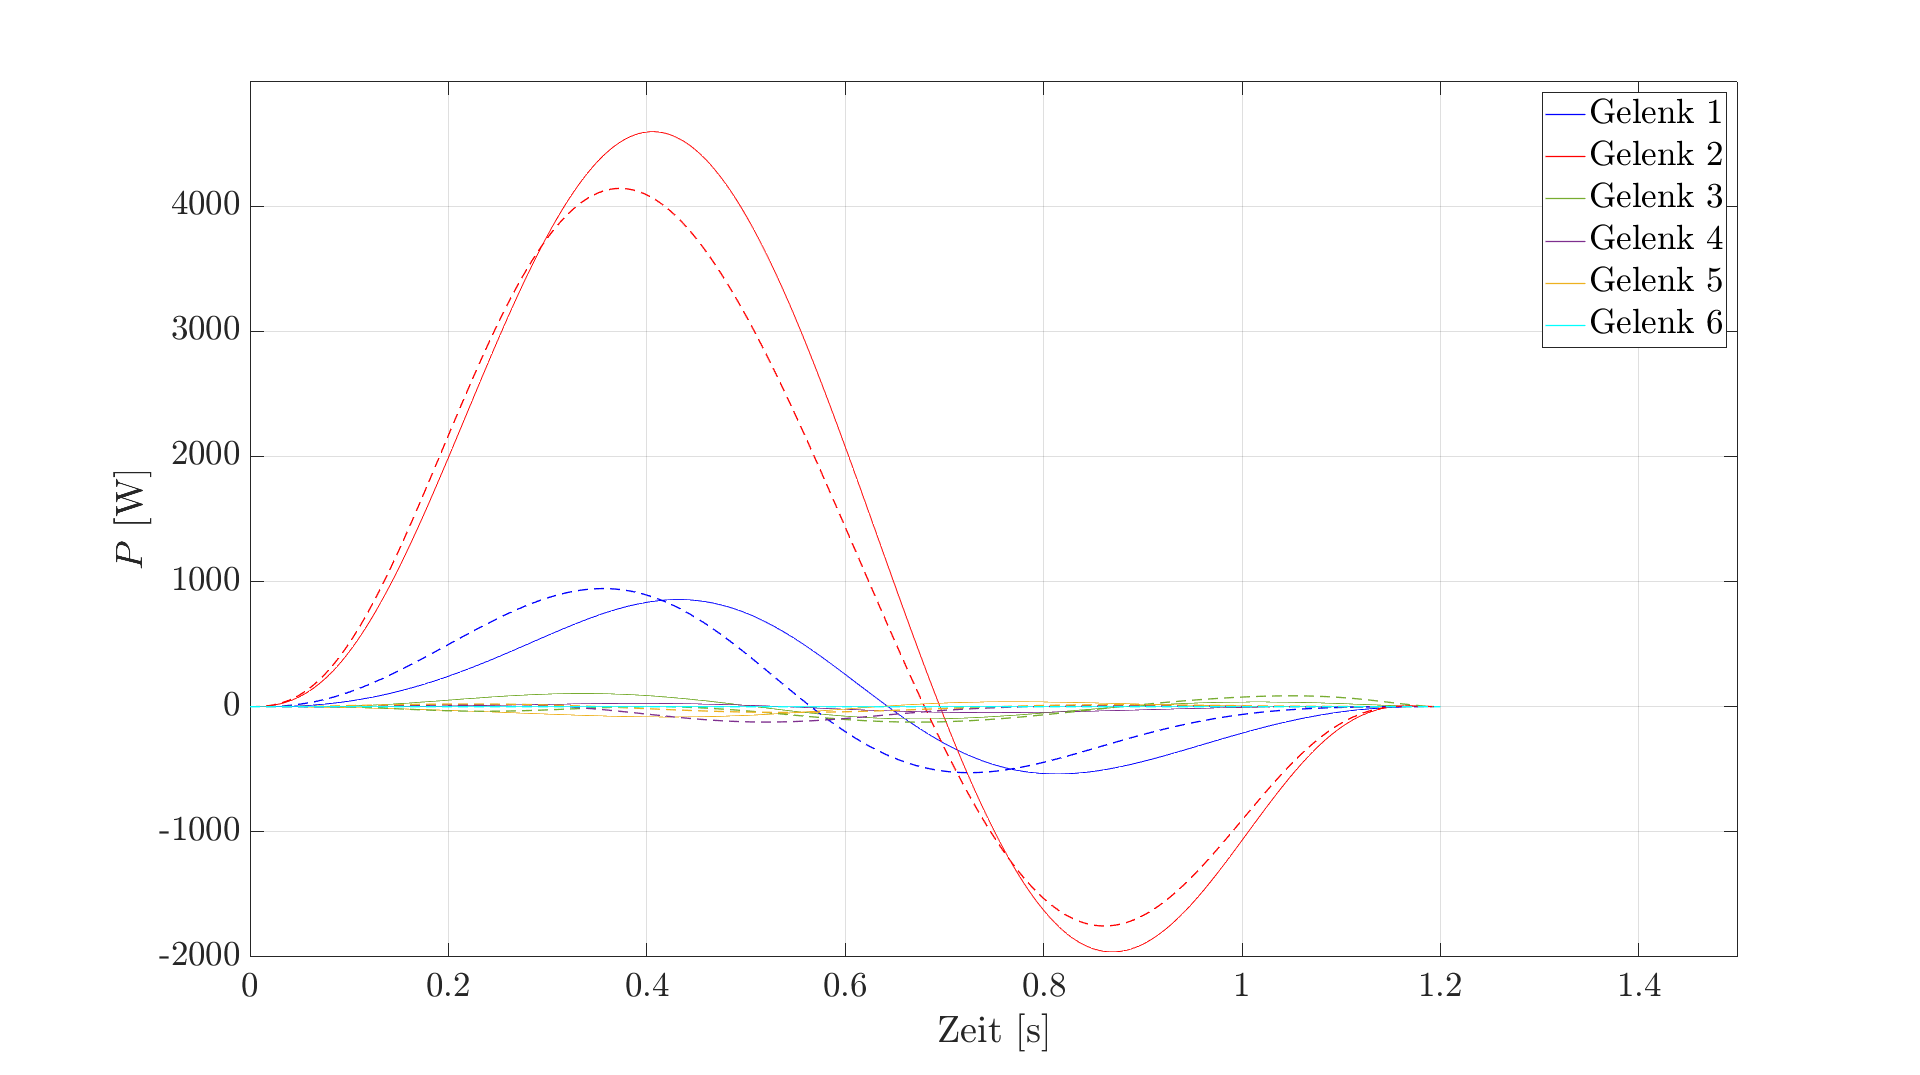
\includegraphics[width=1\linewidth]{images/Optimierungsergebnisse_up/popt}
	\caption{Simulierte Leistungsaufnahme der Initialbahn und optimierten Bewegungsbahn}
	\label{fig:popt}
\end{figure}
%
Nachfolgend werden der Verlauf der Gelenkwinkel in Abbildung \ref{fig:posopt} sowie die Geschwindigkeitsnebenbedingungen in Abbildung \ref{fig:velopt} untersucht. Für den Verlauf des Winkels im zweiten Gelenk ist keine auffällige Abweichungen gegenüber der Initialbahn zu erkennen. Die beiden Verläufe der Gelenkwinkel eins und drei zeigen geringe Differenzen im Bereich der Via-Punkte. Signifikante Unterschiede sind für die Verläufe der Gelenkwinkel vier, fünf und sechs erkennbar.  Bei Betrachtung der Abbildung \ref{fig:velopt} fällt auf, dass die Winkelgeschwindigkeiten $\dot{q}_{4}(t)$, $\dot{q}_{5}(t)$ und $\dot{q}_{6}(t)$ erheblich größer ausfallen als die Originalverläufe. Dies ist auf die Nähe der Gelenkwinkel ${q}_{v,4}$, ${q}_{v,5}$ und ${q}_{v,6}$ zu den Grenzwerten in Kombination mit der Größe des Gelenkwinkelhub $\Delta q_i = | q_{s,i}+q_{e,i} | ~\forall~ i \in \{4,5,6\}$ zurückzuführen. 
%
\begin{figure}[tbph]
	\centering
	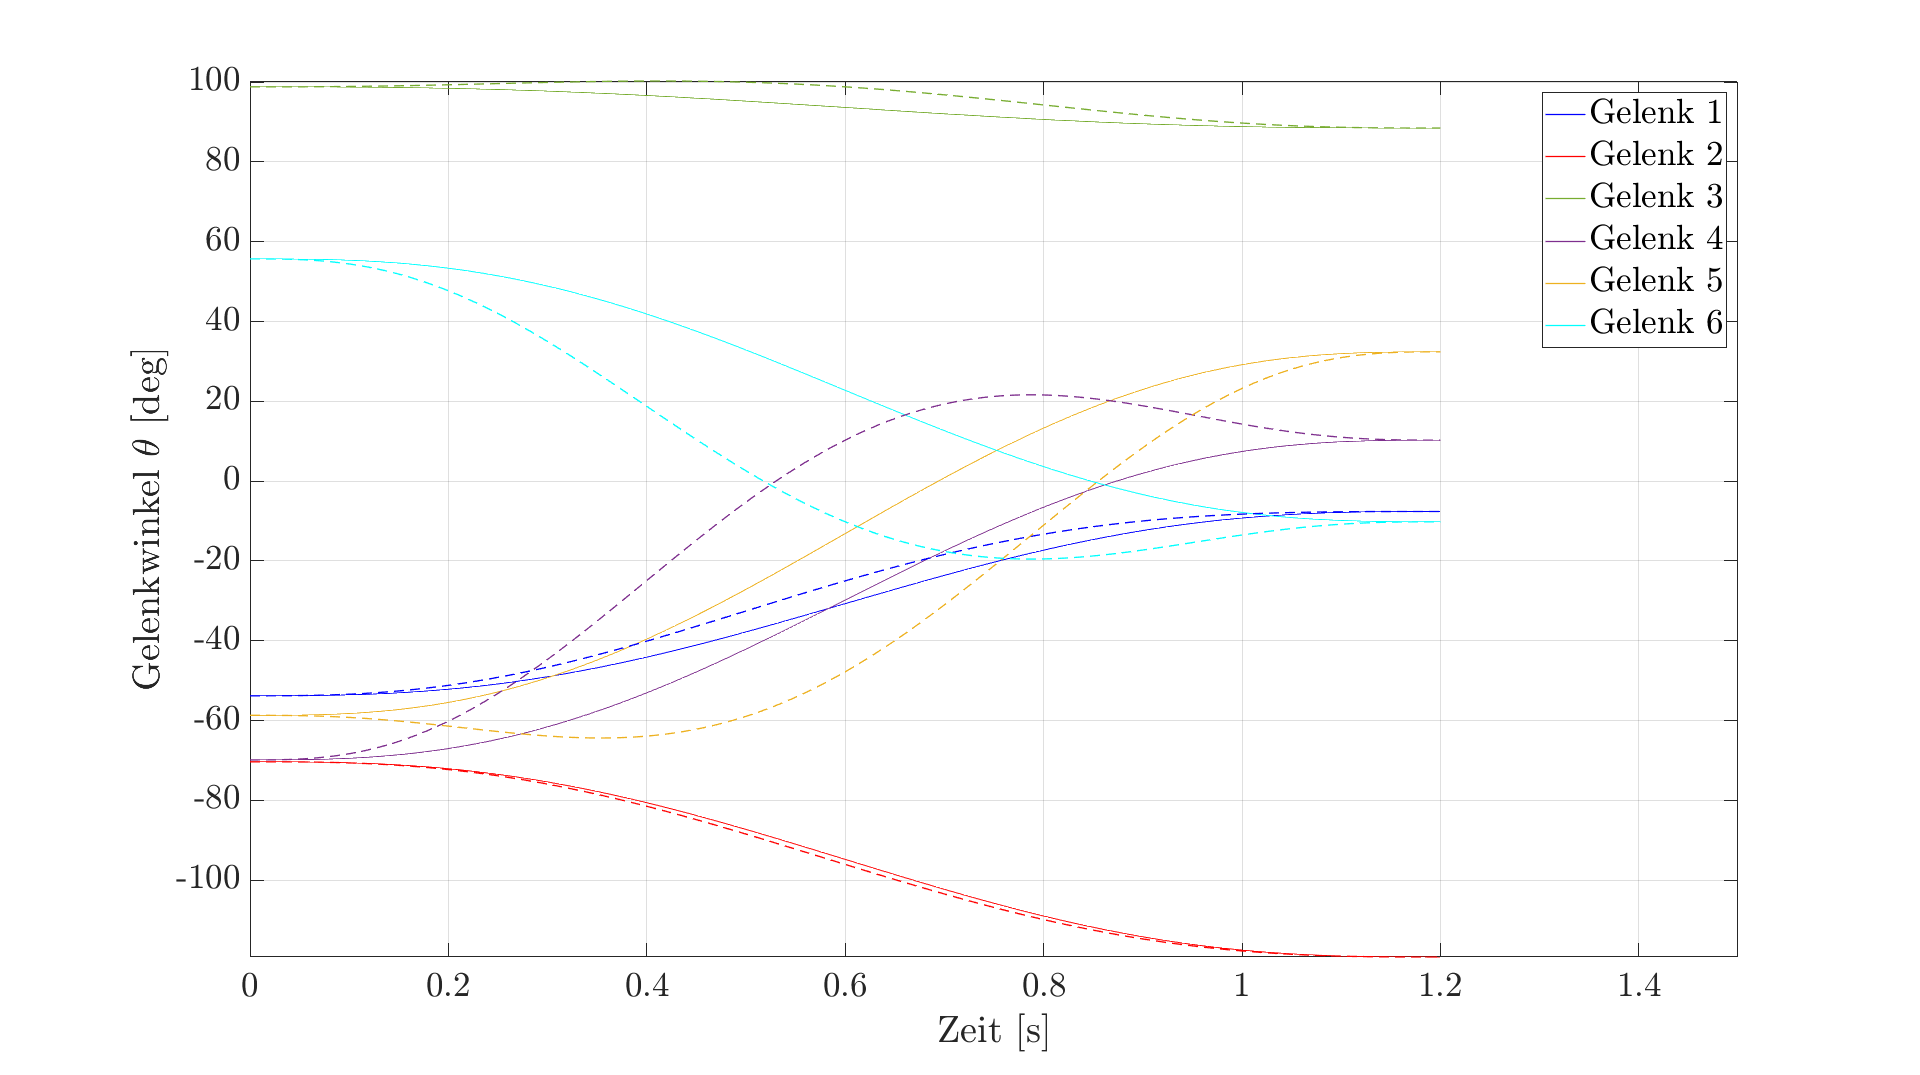
\includegraphics[width=1\linewidth]{images/Optimierungsergebnisse_up/posopt}
	\caption{Gelenkwinkelverläufe der Initialbahn und energieoptimierten Bewegungsbahn}
	\label{fig:posopt}
\end{figure}
%
\begin{figure}[tbph]
	\centering
	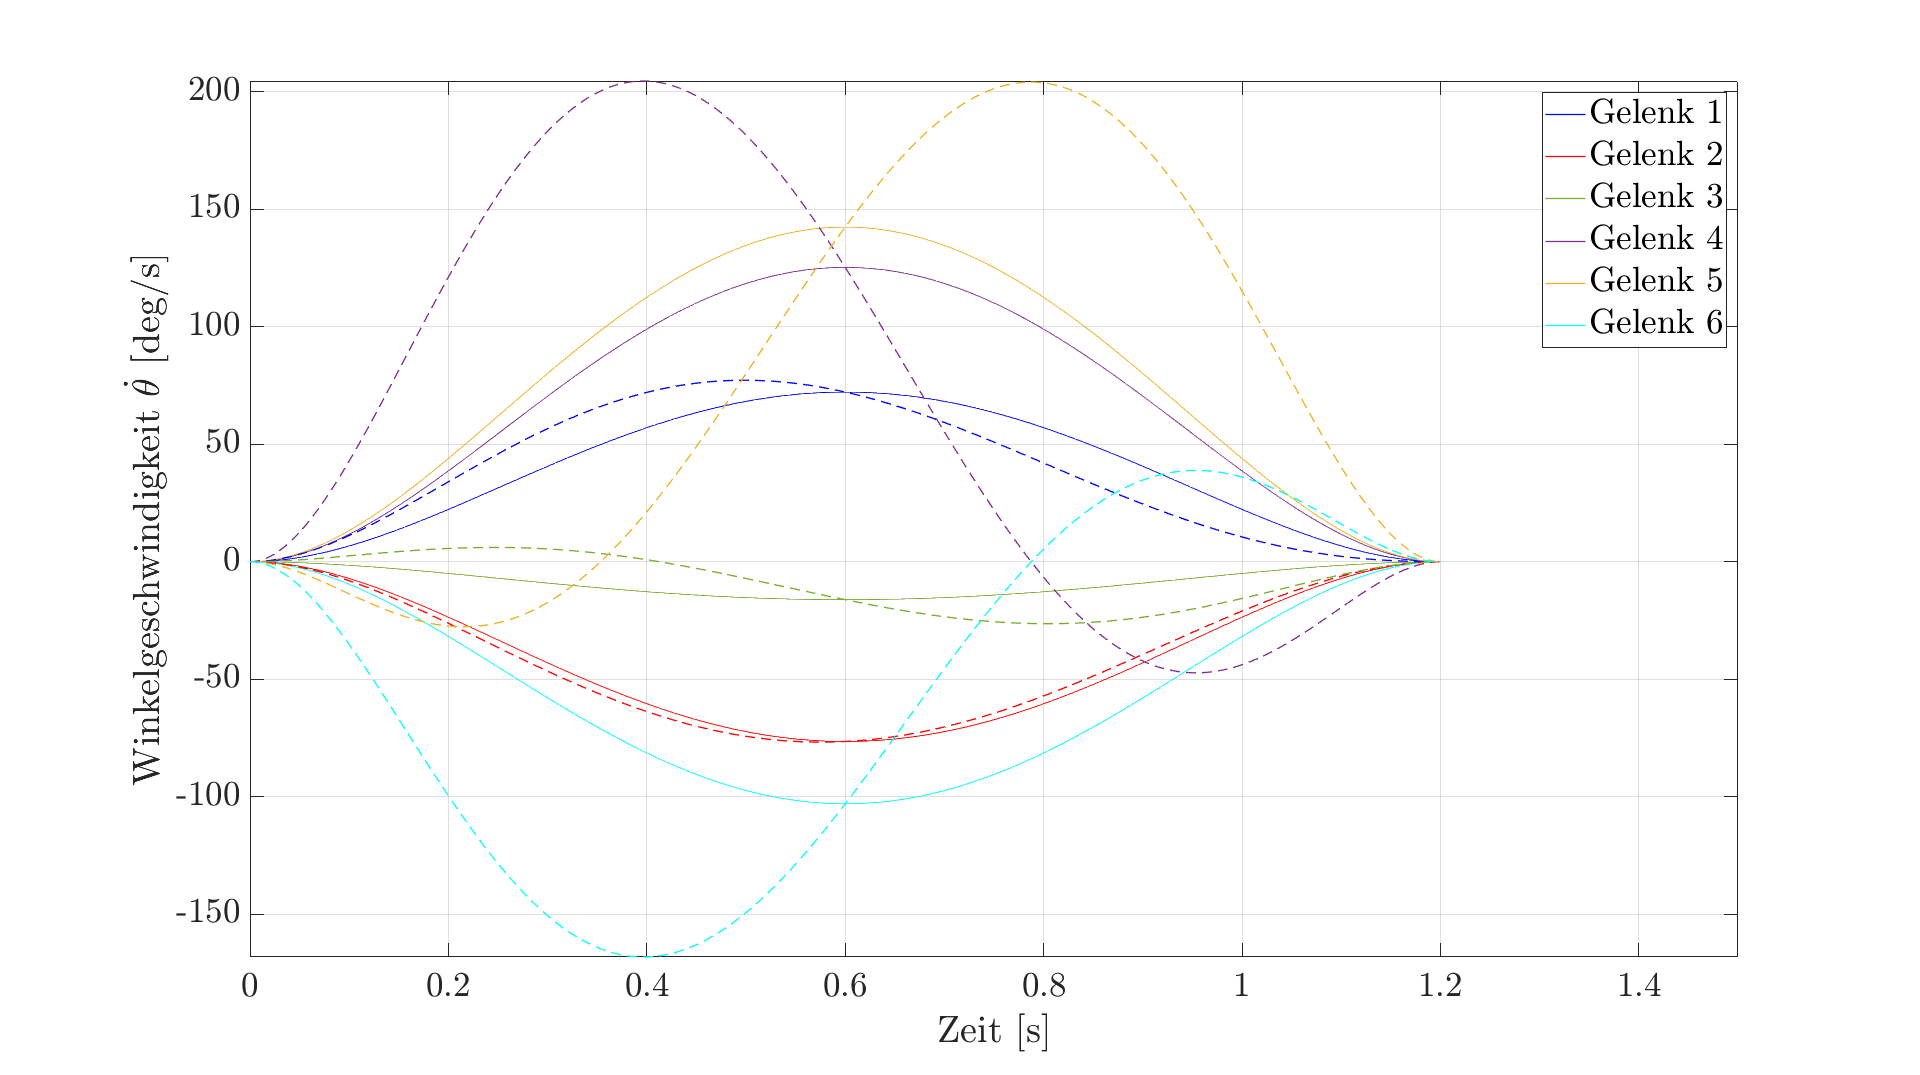
\includegraphics[width=1\linewidth]{images/Optimierungsergebnisse_up/velopt}
	\caption{Winkelgeschwindigkeitsverläufe der Initialbahn und energieoptimierten Bewegungsbahn}
	\label{fig:velopt}
\end{figure}
%
Infolgedessen werden die Via-Punkte ${q}_{v,4}$, ${q}_{v,5}$ und ${q}_{v,6}$ manuell auf den Mittelwert zwischen der initialen Definition und den energieoptimierten Werten, siehe Gleichung \ref{eqn:manuellejustage} nachjustiert.
%
\begin{equation}
	\label{eqn:manuellejustage}
	{q}_{v,i,justiert} = \dfrac{{q}_{v,i,opt} + \dfrac{q_{s,i}+q_{e,i}}{2}}{2}~\forall~ i \in \{4,5,6\}
\end{equation}
%
Die resultierenden Winkelgeschwindigkeiten in Abbildung \ref{fig:veloptedit} 
%und Winkelbeschleunigungen in Abbildung \ref{fig:accoptedit} 
werden damit auf ein akzeptables Maß reduziert. 
Die energieoptimierten Verläufe sind weiterhin gestrichelt dargestellt. Die Kurven der justierten Via-Punkte werden punktiert abgebildet.
%
\begin{figure}[tbph]
	\centering
	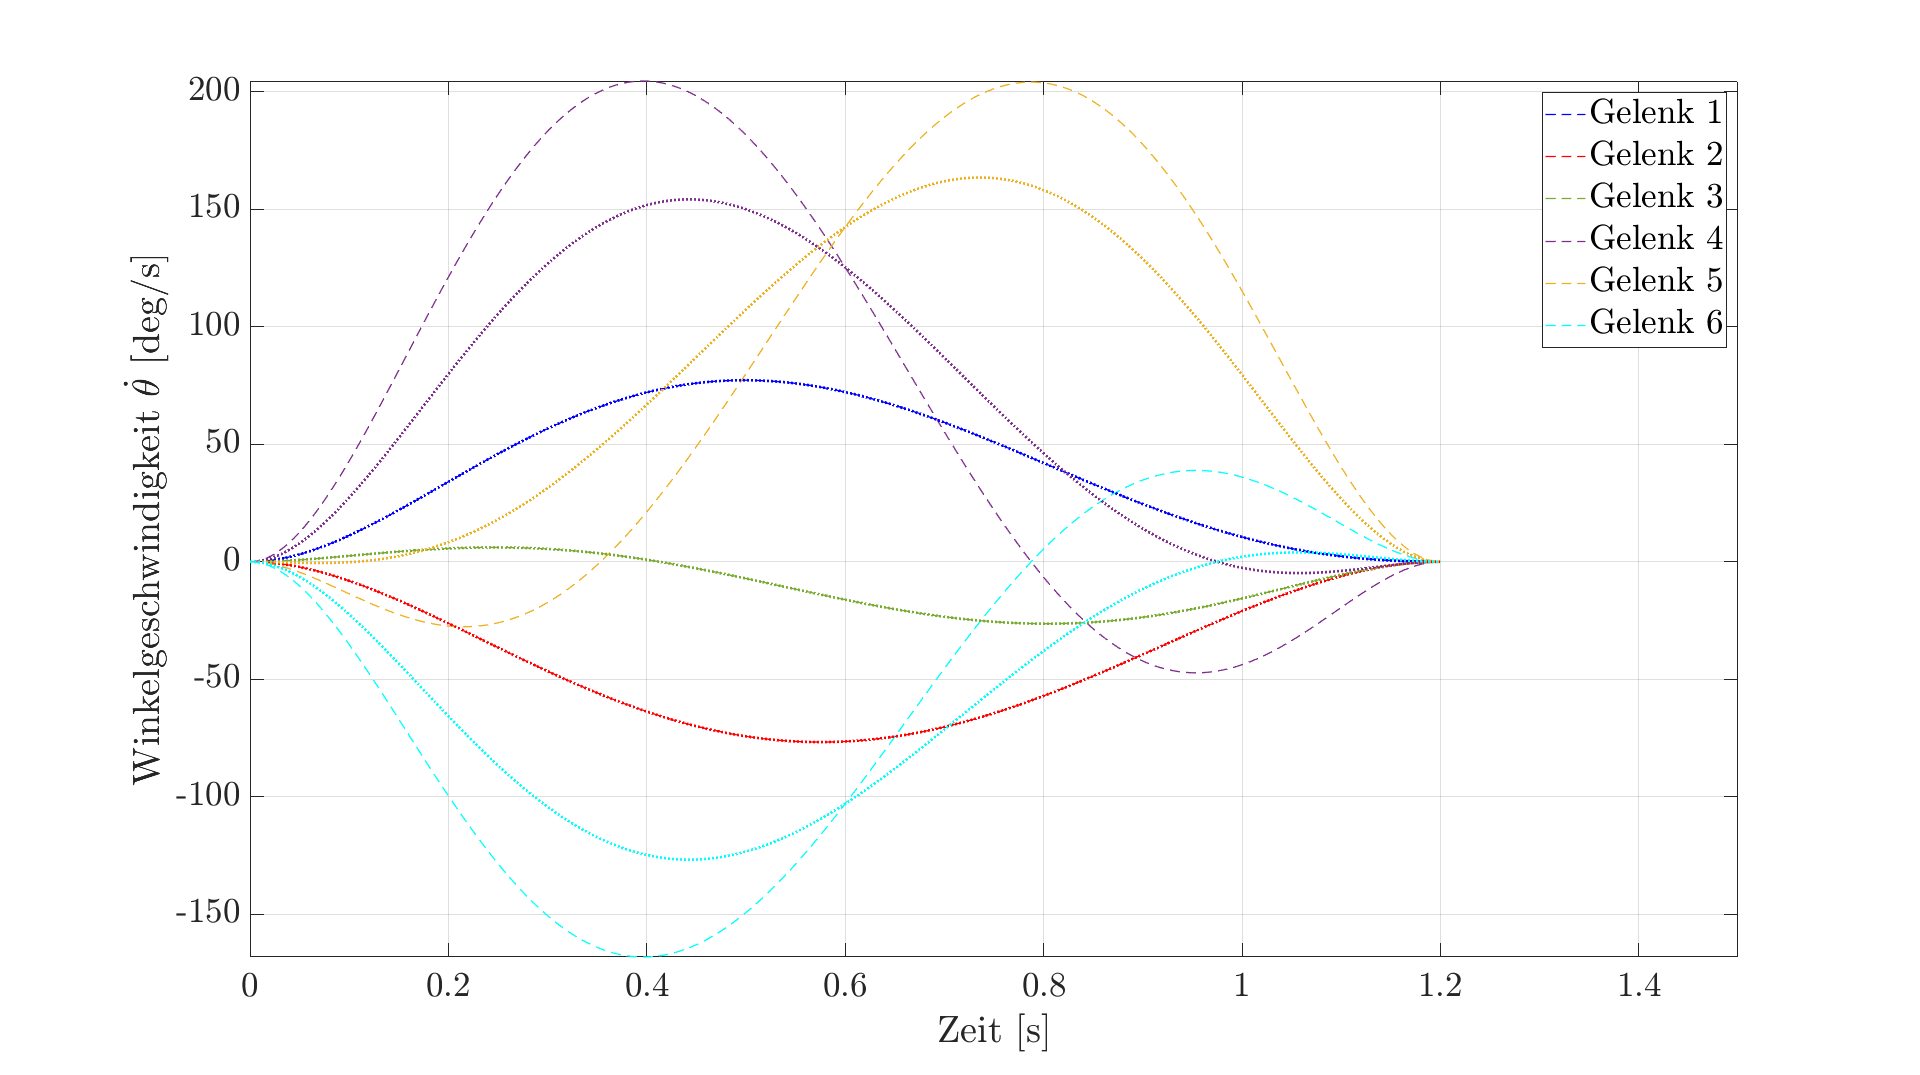
\includegraphics[width=1\linewidth]{images/Optimierungsergebnisse_up/veloptedit}
	\caption{Winkelgeschwindigkeitsverläufe der energieoptimierten Bewegungsbahn und justierten energieoptimierten Bewegungsbahn}
	\label{fig:veloptedit}
\end{figure}
%
%\begin{figure}[tbph]
%	\centering
%	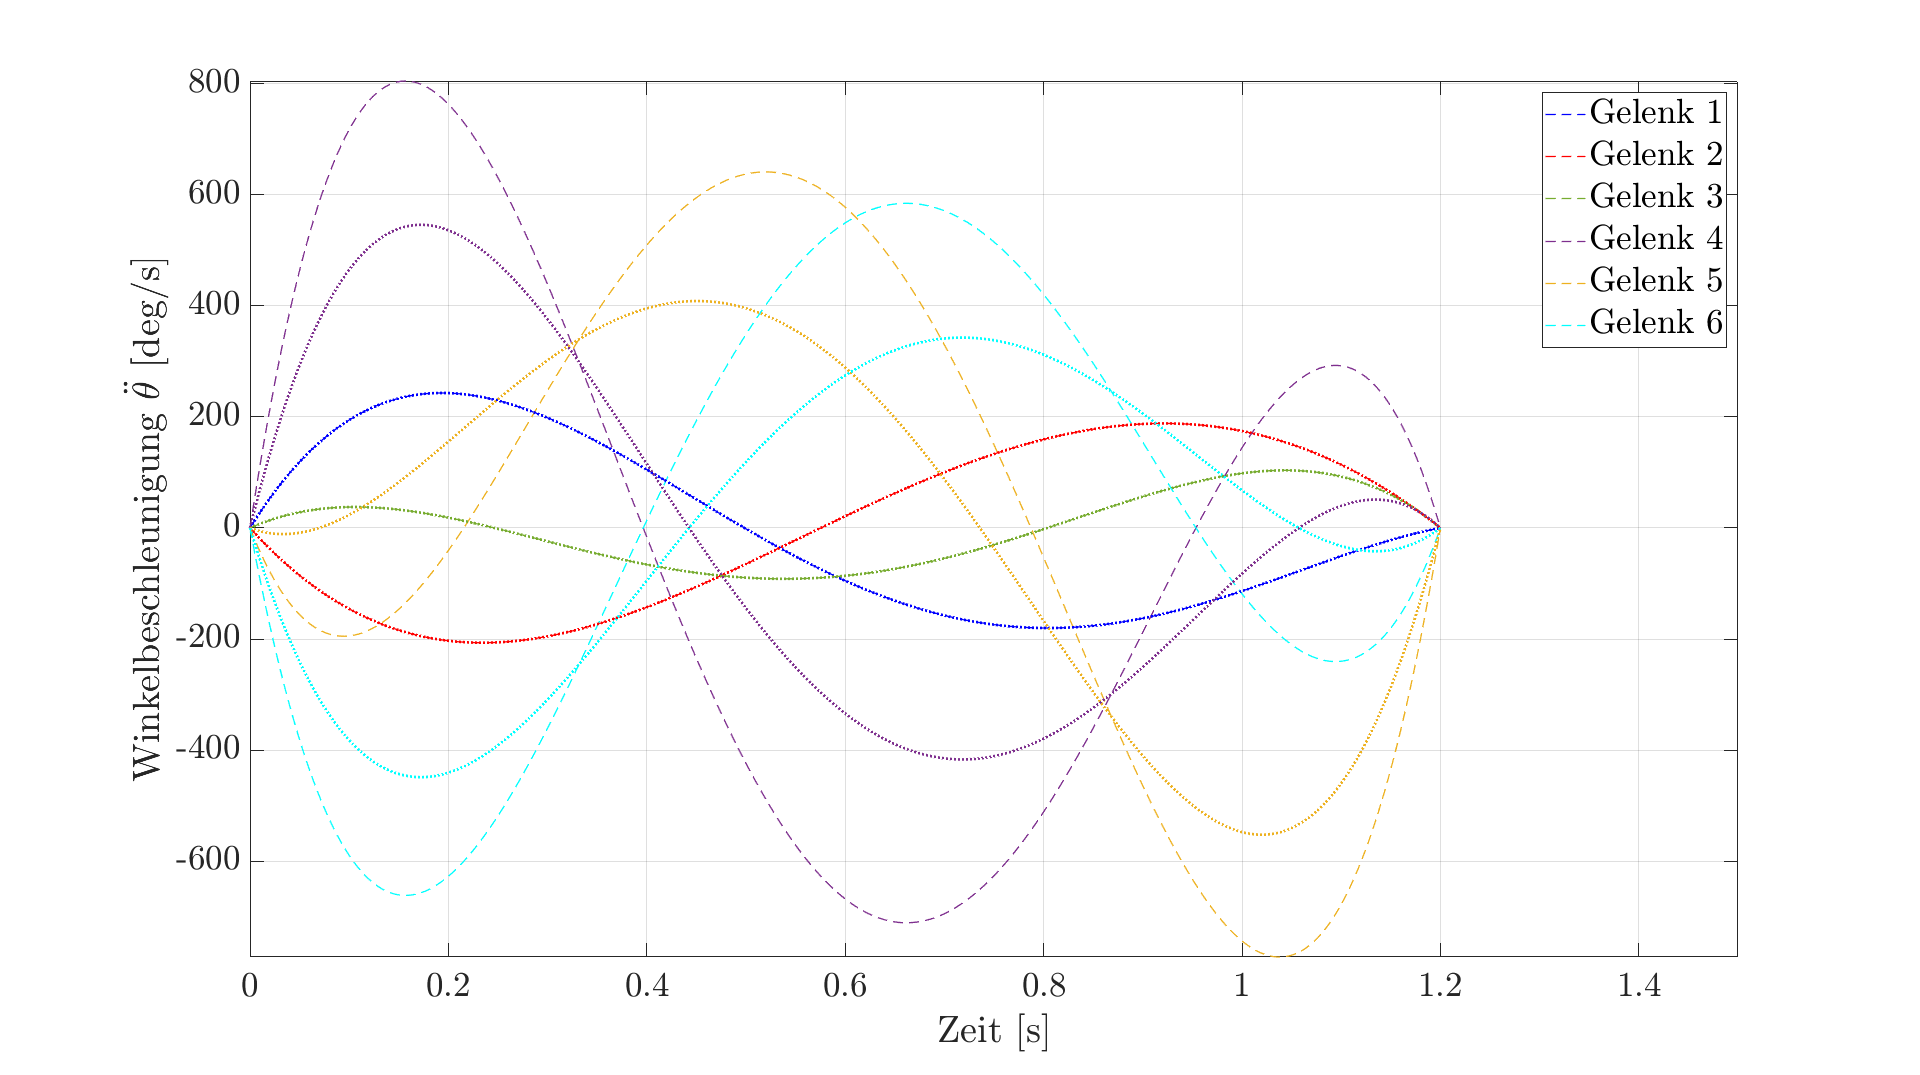
\includegraphics[width=1\linewidth]{images/Optimierungsergebnisse_up/accoptedit}
%	\caption{Winkelbeschleunigungsverläufe der energieoptimierten Bewegungsbahn und justierten energieoptimierten Bewegungsbahn}
%	\label{fig:accoptedit}
%\end{figure}
%
Für den justierten Parametervektor beträgt der Energieverbrauch 1858 Joule. Damit wird eine Energieeinsparung von 7,15 \% gegenüber der Initialbahn erzielt. Der Leistungsverlauf für den justierten Parametervektor wird dem der Initial-Trajektorie in Abbildung \ref{fig:poptfinal} gegenüber gestellt. Der Verlauf entspricht qualitativ dem der  energieoptimierten Bewegungsbahn. Es wird infolge der Anpassung eine leichte Zunahme der Leistungsaufnahme im zweiten Gelenk notiert. Die Gegenüberstellungen der Gelenkwinkel-, Winkelgeschwindigkeits- Beschleunigungs- und Drehmomentverläufe der  initialen- und justierten-Trajektorie sind im Anhang \ref{add:optupjust} aufgeführt.
%
\begin{figure}[tbph]
	\centering
	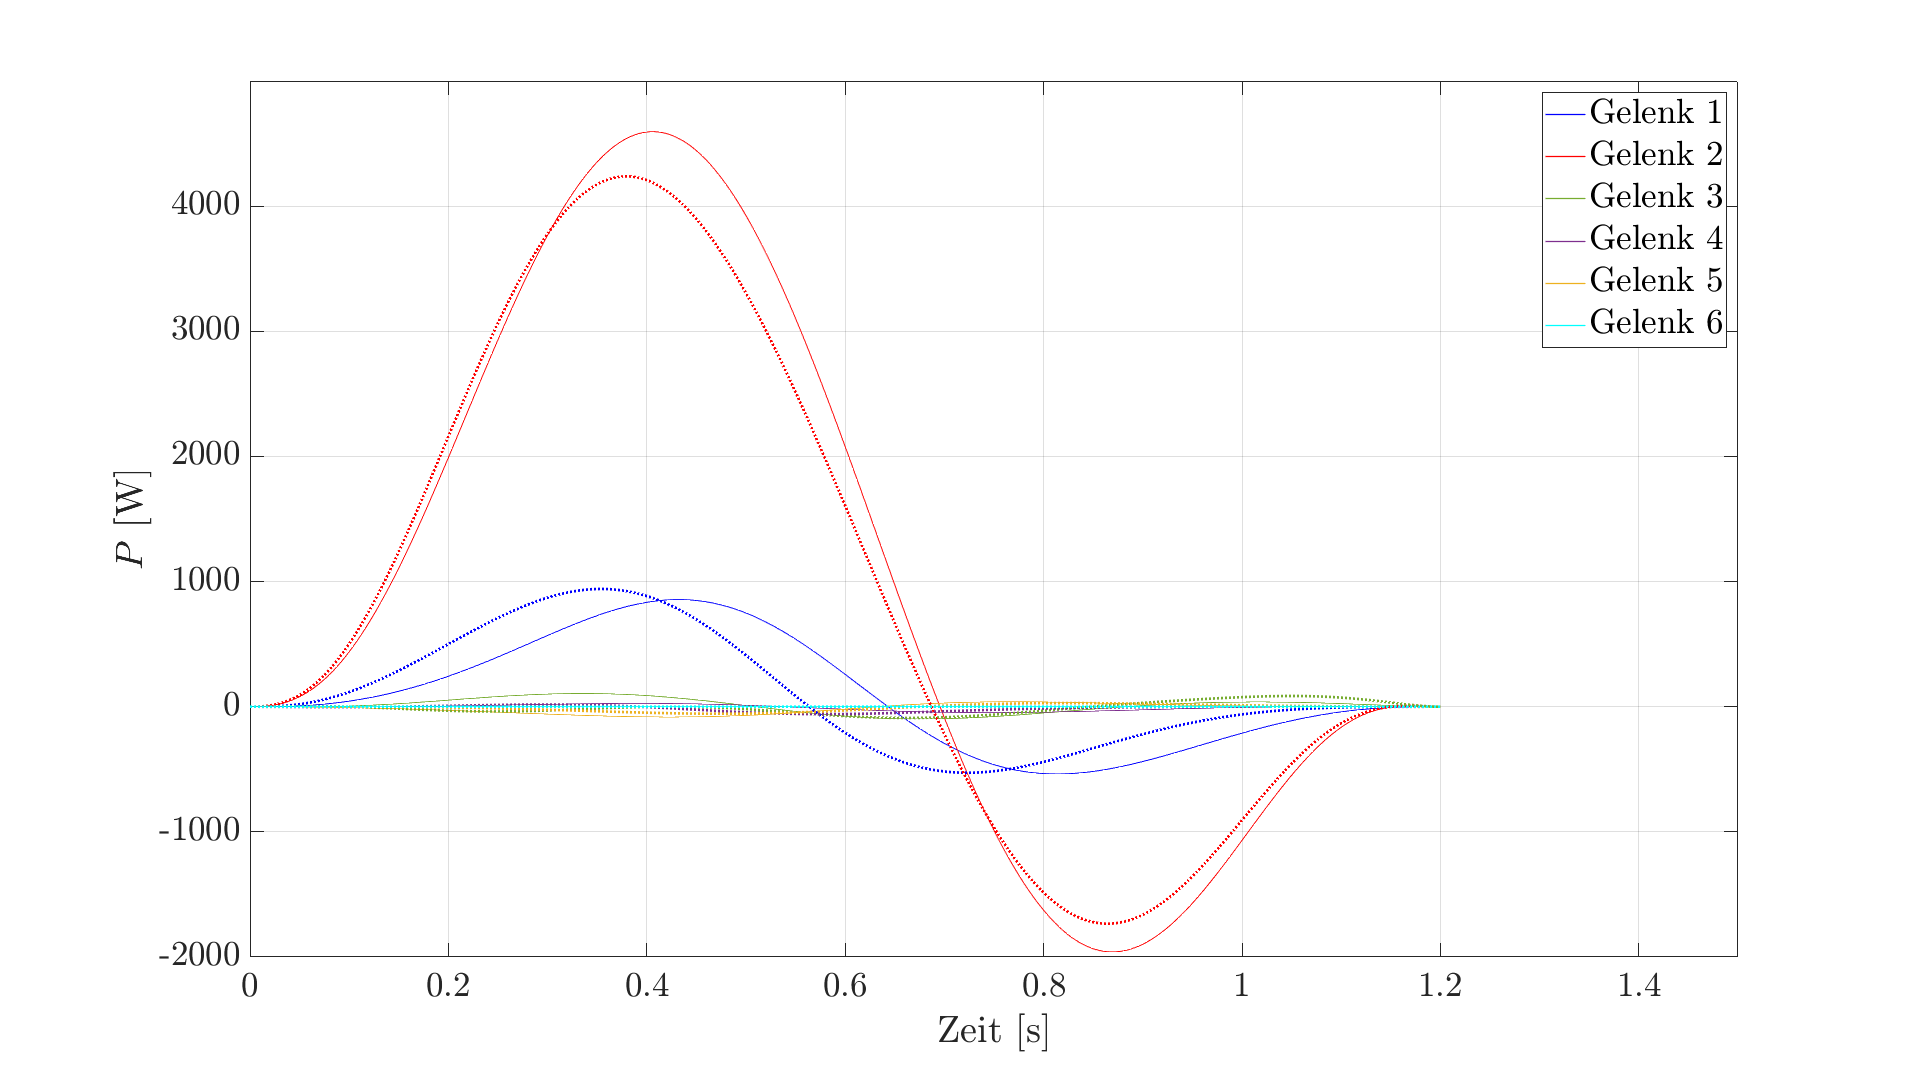
\includegraphics[width=1\linewidth]{images/Optimierungsergebnisse_up/poptfinal}
	\caption{Verläufe der aufgenommen Leistung je Gelenkwinkel für die Initialbahn und justierte-energieoptimierte Bewegungsbahn}
	\label{fig:poptfinal}
\end{figure}
